%% ----------------------------------------------------------------------------
%% article.tex
%% ----------------------------------------------------------------------------

\documentclass[final,3p,times,twocolumn,sort&compress]{elsarticle}
\usepackage[english]{babel}
\usepackage[utf8]{inputenc}
\usepackage[T1]{fontenc}
\usepackage{paralist}
\usepackage{booktabs}
\usepackage{multirow}
\usepackage{subfig}
\usepackage{siunitx}
\usepackage{chemformula}
\usepackage[pdftex, 
			pagebackref=false, 
			linktocpage=true, 
			bookmarksopen=true,
			bookmarksnumbered=true]{hyperref}

% TODO this is not the recommended way of siunitx!
\newcommand{\sccm}{\cubic\centi\metre\per\minute}

% Figures folder is one level above.
\graphicspath{{../figures/}}

\makeatletter 
%workaround for hyperref
%https://www.tug.org/pipermail/tex-live/2012-August/032152.html
\providecommand{\doi}[1]{%
	\begingroup 
	\let\bibinfo\@secondoftwo
	\urlstyle{rm}% 
	\href{http://dx.doi.org/#1}{% 
		doi:\discretionary{}{}{}%
		\nolinkurl{#1}% 
	}% 
	\endgroup } 
\makeatother

\bibliographystyle{elsarticle-num-names}
\journal{Journal of Analytical and Applied Pyrolysis}

\begin{document}
\begin{frontmatter}
	
	%\title{Possibilities and limitations in the simulation of low pressure
		%	carbonitriding}
	
	\title{Acetylene pyrolysis applied to vacuum carburizing: experimental studies and numerical simulation of precursor decomposition}
	
	\author[ijl,irt]{W. Dal'Maz Silva\corref{cor1}}
	\ead{walter.dal-maz-silva@univ-lorraine.fr}
	
	\author[ijl]{J. Dulcy} 
	\ead{jacky.dulcy@univ-lorraine.fr}
	
	\author[irt]{P. Lamesle}
	\ead{pascal.lamesle@irt-m2p.fr}
	
	\author[ijl]{T. Belmonte\corref{cor2}} 
	\ead{thierry.belmonte@univ-lorraine.fr}
	
	\cortext[cor1]{Corresponding author} 
	\cortext[cor2]{Principal corresponding author}
	
	\address[ijl]{Institut Jean Lamour, Parc de Saurupt, Nancy 54011, France}
	\address[irt]{Institut de Recherche Technologique M2P, Metz 57070, France}
	
	\begin{abstract}
		Acetylene pyrolysis has extensively been studied in the last decades due to the large amount of applications of this precursor in several industrial branches. These include deposition processes, vapor infiltration and carburizing of steel among others. A detailed mechanism of hydrocarbon decomposition compiled by \citet{Norinaga2009} and validated for some species as precursors, including acetylene pyrolysis, is studied. Satisfactory results are obtained for the main reaction by-products of \ch{C2H2} decomposition around \SI{1173}{\kelvin} simulated using this mechanism comprised by 241 species and 902 reactions. A modified version of the directed relational graph (DRG) approach by \citet{Lu2005} is used for simplification of this mechanism and results are compared to experimental results. Additionally, chemical graph structure is studied in detail, providing an insightful view of species coupling.
	\end{abstract}
	
	\begin{keyword} 
		acetylene \sep directed relational graph \sep 
		mechanism simplification \sep gas chromatography 
	\end{keyword} 
\end{frontmatter}

\section{Introduction}

Vacuum steel carburizing is a case hardening treatment of mechanical components intended for surface load bearing applications such as power transmission parts and gears. Regarding classical carburizing~\cite{Slycke1981i,Slycke1981ii}, the main difference of the low pressure process is the absence of the oxide layer formed in the partially oxidizing \ch{CO - H2} atmosphere. The process profits from low molecular weight hydrocarbons \textendash{} such as \ch{CH4}, \ch{C2H2}, \ch{C2H4} and \ch{C3H8} \textendash{} as carbon sources and it has been studied from both metallurgical~\cite{Tsuji1987,Liu2003,Kula2005,Kula201326,Gorockiewicz2010429,Gorockiewicz2011,Zajusz2014646} and kinetics~\cite{Iwata2005,Yada2013,Graf2007,Khan2008} standpoints. Although the literature is limited in the description of process kinetics specifically devoted to carburizing, much has been published about its common precursors decomposition~\cite{Benzinger1996957,Becker1998177,Becker1998201,Becker1998213,Becker1998225,Ziegler2005107,Ziegler2005212,Ziegler2005231,Ziegler2005a,Ziegler2007268,Ziegler201348,Khan2008,Norinaga2005,Norinaga2007,Norinaga2007ii,Norinaga2009,Sanchez201230,Sanchez2013126,Bensabath2016} with respect to their sooting characteristics and reaction pathways to undesired species such as polycyclic aromatic hydrocarbons (PAH).

The present work aims at investigating the decomposition of \ch{C2H2} under conditions relevant to vacuum steel carburizing. At first, acetylene decomposition is studied diluted in nitrogen in a vertical tubular flow reactor. These experiments were carried out at atmospheric pressure under partial pressures equivalent to those employed in steel treatment (around \SI{20}{\hecto\pascal}) but with much longer residence times (in the order of \SI{100}{\second}). Reduced pressure studies were carried in an horizontal tubular flow reactor with the same partial pressure range but residence times are reduced to the order of \SI{1}{\second}. Results are confronted to available literature data and compared to both global models~\cite{Zwietering1959,Norinaga2005,Graf2007} and detailed chemical kinetics~\cite{Norinaga2009}. Low pressure results were represented by a plug flow reactor (PFR) given the high flow speeds resulting in an relatively high Péclet number~\cite{Fogler1999}.

Numerical studies were performed with routines implemented with chemical kinetics library Cantera~\cite{Cantera2014} and graph search algorithms from NetworkX~\cite{Networkx2016}. In order to provide a simpler mechanism for future industrial process simulation, \citet{Norinaga2009} mechanism is submitted to directed relational graph (DRG) simplification~\cite{Lu2005,Lu2006i,Lu2006ii,Pepiot2008}. Although the method has been criticized~\cite{Coles2011} and a more feature complete scheme exists such as CSP~\cite{Lam1993,Lam1994,Ortega2007}, it is of simple implementation and interpretation, it has already been employed for our purpose~\cite{Liang2009} and recently was used for automated mechanism simplification~\cite{Curtis2015}. Furthermore, the graph approach allows for mechanism structure analysis~\cite{Toth2015}.

\section{Materials and methods}

\subsection{\label{sec:mat-atmospheric-pressure}Atmospheric pressure experimental setup}

The vertical tubular flow reactor employed in the atmospheric pressure experiments has a diameter of \SI{50}{\milli\metre} and total tube length of \SI{60}{\centi\metre}. Gas injection is performed by a \SI{2}{\milli\metre}-diameter tube with its extremity placed at \SI{25}{\centi\metre} from the reactor top, leading to an equivalent length with restrained gas circulation. Heated zone is \SI{20}{\centi\metre} long and starts \SI{30}{\centi\metre} below the reactor top. Temperature set-point is found to be homogeneous in a length of \SI{10}{\centi\metre} centered in the heated region. The lower part of the reactor is symmetric with the previously described upper part. Reactor outlet is kept at atmospheric pressure and flue gas is partially conducted to a Carlo Erba GC6000 Vega Series 2 gas chromatograph (GC) equipped with both a flame-ionization (FID) and a thermal-conductivity (TCD) detectors for gas characterization.

Atmosphere composition was fixed to \ch{N2 - 0.02 C2H2} (given in mole fractions), leading to a partial pressure of acetylene around \SI{20}{\hecto\pascal}. Heated zone temperature was set between \SIrange{873}{1223}{\kelvin} and total volume flow rates of \SIlist{500;1000}{\cubic\centi\metre\per\minute} were employed. Gas phase hydrocarbons up to \ch{C2} where identified by FID-GC and \ch{H2} by TCD-GC. Probability density functions for different flow rates were measured by the tracer pulse method~\cite{Fogler1999} with the heated zone of the vertical tubular reactor set to \SI{1173}{\kelvin}. Methane was employed as tracer gas given its reasonable stability at operating temperature in the absence of oxygen (no \ch{C2} reaction by-products are observed under the experimental conditions). Injection volume for the pulse was \SI{10}{\milli\litre} (approximately 2.5\% of the heated zone volume). These measurements are intended to suit the needs of a global decomposition order analysis at long residence times ($\tau_{eff}>\SI{50}{\second}$).

\subsection{Reduced pressure experimental setup}

Low pressure studies were carried in a horizontal quartz tubular flow reactor of \SI{80}{\centi\metre} in length and diameter of \SI{28}{\milli\metre}. Gas injection is performed \SI{20}{\centi\metre} before the arrival to heated zone in order to ensure a fully established flow in this region. Temperature is controlled over a length of \SI{40}{\centi\metre}, the remaining of the tube leading to the outlet and gas chromatography system. Figure~\ref{fig:temperature-profile} presents the actual wall temperature profile measured with a type-K thermocouple along the reactor axis. Gas phase pyrolysis products were analyzed using a Perkins Elmer GC system equipped with a TCD and a gas compression system adapted the GC for low pressure sampling. Separated species comprise \ch{C2H2}, \ch{CH4}, \ch{C2H4}, \ch{C2H6}, \ch{CO} and \ch{N2}. Assuming that \ch{N2} does not take part in the pyrolysis mechanism other than a third-body, its outlet mole fraction can be used to estimate actual residence time $\tau_{eff}$ and changes in volume flow rate due to average molar mass change.

Pyrolysis was studied with an atmosphere composed of \ch{N2 - 0.36 C2H2} (given in mole fractions) in the temperature range of \SIrange{773}{1273}{\kelvin} and total pressures of \SIrange{30}{100}{\hecto\pascal}. Reference atmospheric volume flow rates were set in the range from \SIrange{222}{378}{\cubic\centi\metre\per\second}. These conditions lead to acetylene partial pressures in the range of \SIrange{11}{36}{\hecto\pascal}.

\subsection{Computational methods and tools}

Global order analysis coupled to residence time distribution (RTD) was carried for atmospheric pressure decomposition of \ch{C2H2}. These estimations considered decomposition to take place in the homogeneous temperature region of the reactor. It is proposed that the RTD of this region can be approximated by the peak and decay tail of the approximately tubular flow reactor measured distribution (the delay before the peak can be attributed to a plug-like behavior after the heated zone) as shown in Fig.~\ref{fig:residence-time-plot}. Acetylene conversion was computed with aid of RTD data by assuming a maximum mixedness model originally attributed to \citet{Zwietering1959}.

Reduced pressure results were represented by a plug-flow reactor (PFR) model implemented with the Python interface of chemical kinetics library Cantera~\cite{Cantera2014}. This model assumption is reasonable given the  Péclet number $\mathrm{Pe}\gg{}1$ which can be computed for the system\footnote{See generated simplified mechanism file. The computation of Péclet number $\mathrm{Pe}\approx{}300$ considered the average diffusivity \textendash{} provided by Cantera~\cite{Cantera2014} using Lennard-Jonnes model \textendash{} of all species at \SI{1173}{\kelvin} and \SI{5000}{\pascal}.}. Tube length is divided in small lengths $\delta$, each being represented by a perfect stirred reactor (PSR) model. The first reactor is fed with the inlet gas and its steady-state solution is then employed to feed the next reactor in the network and so on until the whole length is covered. Discretization length $\delta$ was reduced until the relative difference between consecutive outlet solutions for selected species (\ch{C2H2}, \ch{H2}, \ch{C2H4}, \ch{C4H4} and \ch{C6H6}) fall below $10^{-6}$. 

A detailed mechanism assembled by \citet{Norinaga2009} was used for the first set of simulations. Inlet \ch{N2} was assumed to be free from contaminants, while \ch{C2H2} composition took into account recommended values~\cite{Norinaga2007} of impurities, as given in Tab.~\ref{tab-acetylene-inlet-composition}. In order to represent actual temperature profiles, convective heat transfer was added to the simulations by considering a constant local wall temperature (Nusselt number $\mathrm{Nu}=3.66$) and global heat transfer coefficient $\bar{U}=k\,\mathrm{Nu}\,\delta^{-1}$. Gas thermal conductivity was computed using a mixing model with Cantera~\cite{Cantera2014} built-in functions.

\begin{table}[h]
	\caption{\label{tab-acetylene-inlet-composition}Inlet acetylene gas composition given in mole fractions adopted for simulations. Nitrogen carrier is assumed free of impurities and its proportion in the mixture is identical to the experimental conditions.}
	
	\resizebox{\linewidth}{!}{%
		\centering{}\footnotesize{}
		\begin{tabular}{ccc}
			\toprule
			\multicolumn{1}{p{0.3\linewidth}}{\centering\ch{C2H2}}
			& \multicolumn{1}{p{0.3\linewidth}}{\centering\ch{CH3COCH3}}
			& \multicolumn{1}{p{0.3\linewidth}}{\centering\ch{CH4}}
			\tabularnewline
			\midrule
			\multicolumn{1}{c}{0.980}
			& \multicolumn{1}{c}{0.018}
			& \multicolumn{1}{c}{0.002}
			\tabularnewline
			\bottomrule
	\end{tabular}}
\end{table}

For mechanism simplification, \citet{Lu2005} method was implemented in Python with NetworkX~\cite{Networkx2016} graph library. For the computation of relative species interaction terms of the directed relational graph (DRG), Cantera~\cite{Cantera2014} was again employed. By using a fixed atmosphere composition, isothermal PSR integration were carried out at different pressures to obtain a sampling space of solutions for relative interaction parameters computation. Under all circumstances above, kinetics and state equations were integrated with Sundials~\cite{Hindmarsh2005} ordinary differential equation solver CVode.

In order to verify the accuracy and proper functioning of the simplified mechanism here proposed, the system was simulated in 2-D using OpenFOAM~\cite{Weller1998} on its version 5.0 with solver \emph{reactingFoam}. System pressure was set to \SI{5000}{\pascal} and heated zone temperature to \SI{1173}{\kelvin}. Inlet velocity was set to match the flow of \ch{N2 - 0.36 C2H2} at \SI{298}{\kelvin} with a flow rate of \SI{222}{\cubic\centi\metre\per\minute}.

\section{Results and discussion}

\begin{table*}[ht]
	\caption{\label{tab-initial-conditions}Acetylene decomposition conditions.}
	
	\resizebox{\textwidth}{!}{%
		\centering{}\footnotesize{}
		\begin{tabular}{cccccc}
			\toprule
			\multirow{2}{0.15\textwidth}{\centering%
				\textbf{Inlet composition}}
			& \multicolumn{1}{p{0.15\textwidth}}{\centering%
				\textbf{Pressure}}
			& \multicolumn{1}{p{0.15\textwidth}}{\centering%
				\textbf{Total flow rate}}
			& \multicolumn{1}{p{0.15\textwidth}}{\centering%
				\textbf{Temperature}}
			& \multicolumn{2}{c}{\centering%
				\textbf{\ch{C2H2} mole fraction}}
			\tabularnewline
			% EMPTY
			& (\si{\hecto\pascal})
			& (\si{\cubic\centi\metre\per\minute})
			& (\si{\kelvin})
			& \multicolumn{1}{p{0.15\textwidth}}{\centering{}measured}
			& \multicolumn{1}{p{0.15\textwidth}}{\centering{}computed}
			\tabularnewline
			\midrule
			\multirow{13}{0.15\textwidth}{\centering{}\ch{N2 - 0.02 C2H2}}
			& \multirow{13}{0.15\textwidth}{\centering{}$1000$}
			& \multirow{8}{0.15\textwidth}{\centering{}$500$}  
			&   $873$  & 0.020768 & 0.019565 \tabularnewline
			&&& $923$  & 0.017902 & 0.017578 \tabularnewline
			&&& $973$  & 0.014093 & 0.014423 \tabularnewline
			&&& $1023$ & 0.010813 & 0.010981 \tabularnewline
			&&& $1073$ & 0.007953 & 0.008045 \tabularnewline
			&&& $1123$ & 0.005995 & 0.005836 \tabularnewline
			&&& $1173$ & 0.004247 & 0.004259 \tabularnewline
			&&& $1223$ & 0.003131 & 0.003151 \tabularnewline
			\cmidrule{3-6}
			&& \multirow{5}{0.15\textwidth}{\centering{}$1000$} 
			&   $1023$ & 0.013880 & 0.013431 \tabularnewline
			&&& $1073$ & 0.010945 & 0.010310 \tabularnewline
			&&& $1123$ & 0.008762 & 0.007714 \tabularnewline
			&&& $1173$ & 0.006963 & 0.005744 \tabularnewline
			&&& $1223$ & 0.005377 & 0.004307 \tabularnewline
			\midrule
			\multirow{15}{0.15\textwidth}{\centering{}\ch{N2 - 0.36 C2H2}}
			& \multirow{3}{0.15\textwidth}{\centering{}$30$}
			& \multirow{3}{0.15\textwidth}{\centering{}$222$}
			&   $1123$ & & \tabularnewline
			&&& $1173$ & & \tabularnewline
			&&& $1223$ & & \tabularnewline
			\cmidrule{2-6}
			& \multirow{7}{0.15\textwidth}{\centering{}$50$}
			& \multirow{7}{0.15\textwidth}{\centering{}$222$}
			&   $773$  & & \tabularnewline
			&&& $873$  & & \tabularnewline
			&&& $973$  & & \tabularnewline
			&&& $1023$ & & \tabularnewline
			&&& $1073$ & & \tabularnewline
			&&& $1123$ & & \tabularnewline
			&&& $1173$ & & \tabularnewline
			&&& $1273$ & & \tabularnewline
			\cmidrule{2-6}
			& \multirow{5}{0.15\textwidth}{\centering{}$100$}
			& \multirow{3}{0.15\textwidth}{\centering{}$222$}
			&   $1173$ & & \tabularnewline
			&&& $1223$ & & \tabularnewline
			&&& $1273$ & & \tabularnewline
			\cmidrule{3-6}
			&& \multirow{2}{0.15\textwidth}{\centering{}$378$}
			&   $1023$ & & \tabularnewline
			&&& $1123$ & & \tabularnewline
			\bottomrule
	\end{tabular}}	
\end{table*}

\subsection{Atmospheric pressure decomposition}

The resulting decomposition of diluted hydrocarbons at atmospheric pressure as described in Section \ref{sec:mat-atmospheric-pressure} are presented in Figures~\ref{fig:fractions-atmospheric-pressure-main}~and~\ref{fig:fractions-atmospheric-pressure-other}.
Acetylene (\ch{C2H2}) decomposition is depicted in Fig.~\ref{fig:fractions-atmospheric-pressure-main} showing that at \SI{873}{\kelvin}, the lowest temperature employed in the study of atmospheric pressure pyrolysis, the compound remains stable during the experiment time-scale and thus measurements were carried only for low total flow rate (\SI{500}{\sccm}). A temperature increase of just \SI{50}{\kelvin} with respect to this reference stability point is enough to start decomposition, which is observed to increase rapidly with temperature. Since experiments were carried under same room temperature flow rate but at different temperatures, no direct kinetic exploitation can be done to check measurement accuracy. One can start this verification by assuming acetylene pyrolysis follows a second order global path, as well established in the literature. Assuming that the system behaves as a stirred reactor with small volume change due to decomposition of acetylene in the mixture \textendash{} thus inlet flow rate $\dot{Q}_{in}$ equals outlet flow rate $\dot{Q}_{out}$, or simply $\dot{Q}$ \textendash{} and a quick approach of thermal steady state, an Arrhenius rate constant $k(T)$ can be adjusted to experimental data by optimizing the mole balance Eq.~\ref{equ:optimize-constant} below

\begin{equation}
	\dot{Q}\,C^{0}_{Ac} - \dot{Q}\,C^{\infty}_{Ac}-
	2\,k(T)\,C^{\infty}_{Ac} = 0
	\label{equ:optimize-constant}
\end{equation}

\noindent{}where inlet \ch{C2H2} composition is given by $C^{0}_{Ac}$ and its measured steady-state counterpart by $C^{\infty}_{Ac}$. It must be emphasized that flow rate $\dot{Q}$ needs to be corrected to take into account the expansion from room to operating temperature\footnote{Thus, setup flow rate has to be multiplied by the ratio of reactor and room temperatures.}. This procedure provides a rate constant given by Eq.~\ref{equ:acetylene-global rate} in units of \si{\cubic\centi\metre\per\mole\per\second}. Both rate pre-exponential factor and activation energy in this constant match the order of magnitude of those for reactions \ch{C2H2 + C2H2 <=> C4H4} and \ch{C2H2 + C2H2 <=> C4H2 + H2} as reported by \citet{Norinaga2009}, and thus the measurements are validated. Table \ref{tab-initial-conditions} presents the measured outlet acetylene mole fractions from Fig.~\ref{fig:fractions-atmospheric-pressure-main} alongside the values computed by integrating a second order process of pyrolysis with the aforementioned assumptions. Error is expected to be greater for \SI{1000}{\sccm} since it is possible that the flow rate is high enough so that gas does not attain homogeneous setup temperature.

\begin{equation}
	k(T) = 1.36\times{}10^{11}\exp\left[\frac{-179,180}{RT}\right]
	\label{equ:acetylene-global rate}
\end{equation}

In the range of temperatures from \SIrange{873}{973}{\kelvin} small quantities of the measured by-products (\ch{H2}, \ch{CH4} and \ch{C2H4}) are detected, although the conversion of \ch{C2H2} is around 30\%. This could possibly be explained by the well known starting reaction of acetylene pyrolysis under the considered conditions, \ch{C2H2 + C2H2 <=> C4H4}. The parallel process explaining the formation of the small quantities of \ch{H2} may be linked to the reaction \ch{C2H2 + C2H2 <=> C4H2 + H2}. Regarding the numerical analysis of the pyrolysis process, it is expected that the maximum stiffness of the rate equations for the studied conditions be found somewhere between \SIlist{973;1023}{\kelvin} once it represents a rapid increase in pyrolysis advance.

%TODO perform sensitivity analysis to show that in this range the polymerisation reaction is prevalent.

\begin{figure}[h]
	\centering
	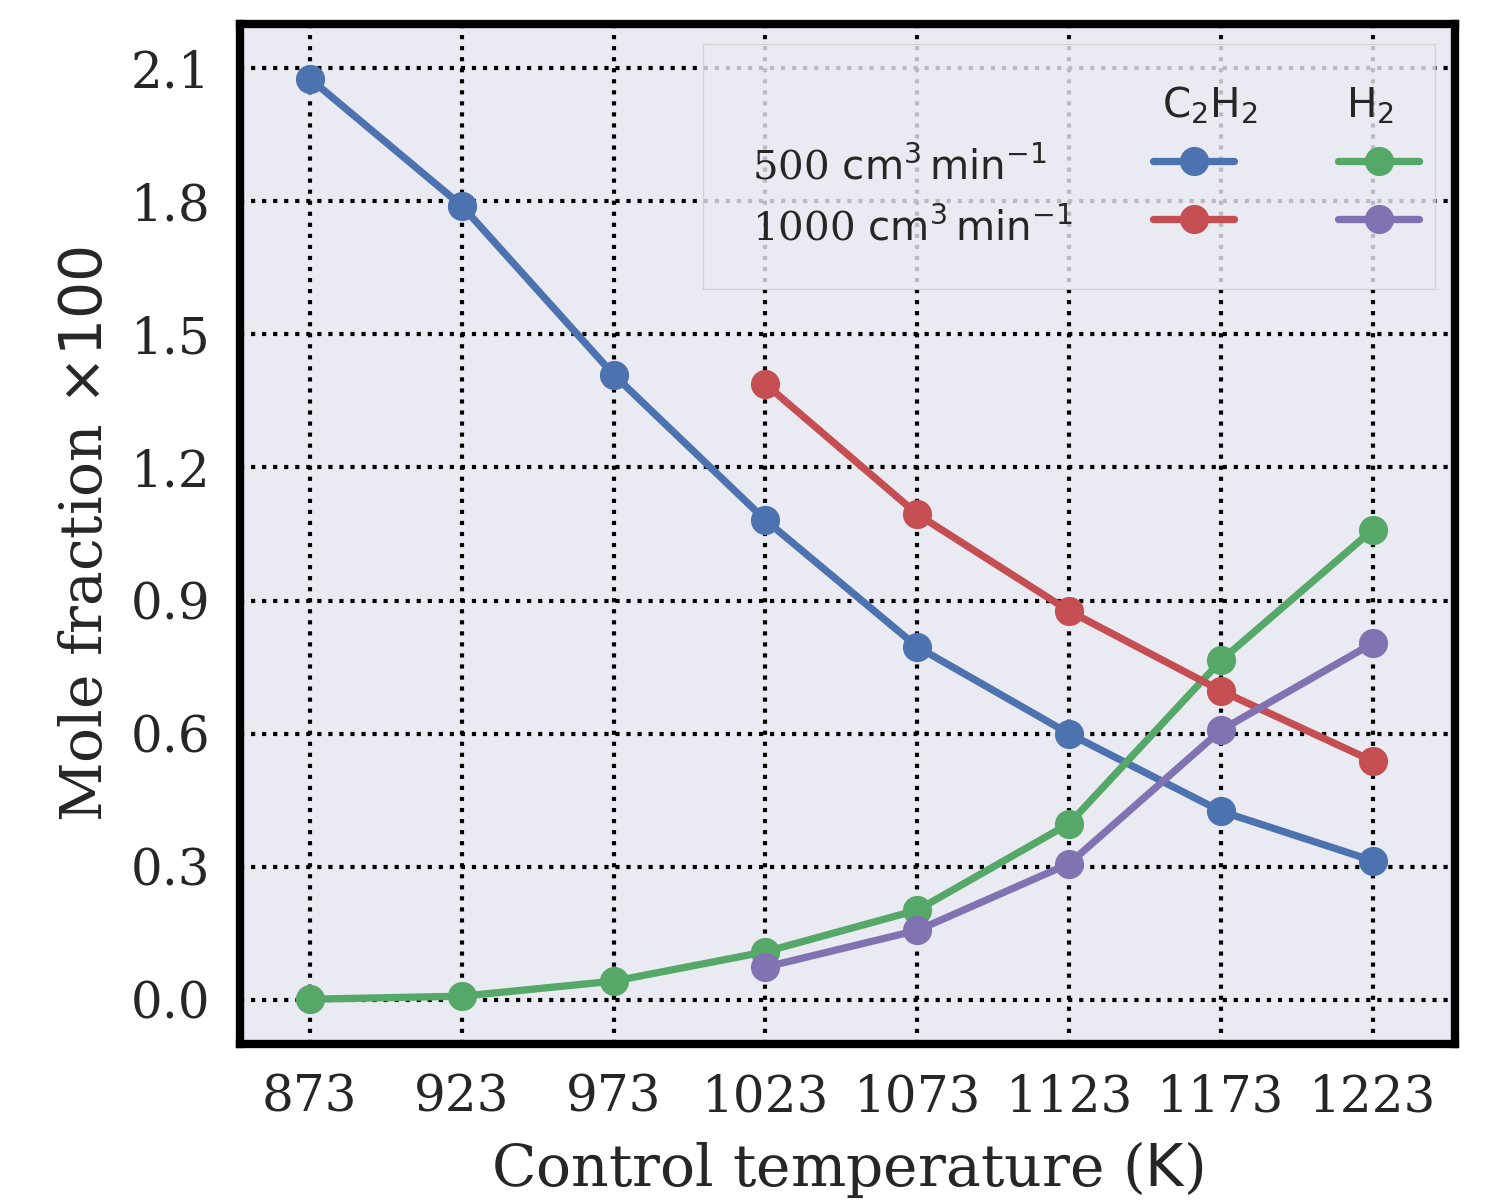
\includegraphics[width=\linewidth]
	{reworking/fractions_atmospheric_pressure_main}
	\caption{\label{fig:fractions-atmospheric-pressure-main}Measured mole fractions of \ch{C2H2} and \ch{H2} at atmospheric pressure in terms of heated zone control temperature for different flow rates.}
\end{figure}

Another important feature is the temperature for which \ch{CH4} and \ch{C2H4} reach an apparent maximum in Figure~\ref{fig:fractions-atmospheric-pressure-other}. While at lower temperatures the main reaction pathways of acetylene decomposition lead to polycyclic aromatic hydrocarbons (PAH), above \SI{1173}{\kelvin} sooting also becomes important and hydrogen release with consumption of low molecular weight species are accelerated. For applications such as vacuum steel carburizing this temperature represents a technological limit.

\begin{figure}[h]
	\centering
	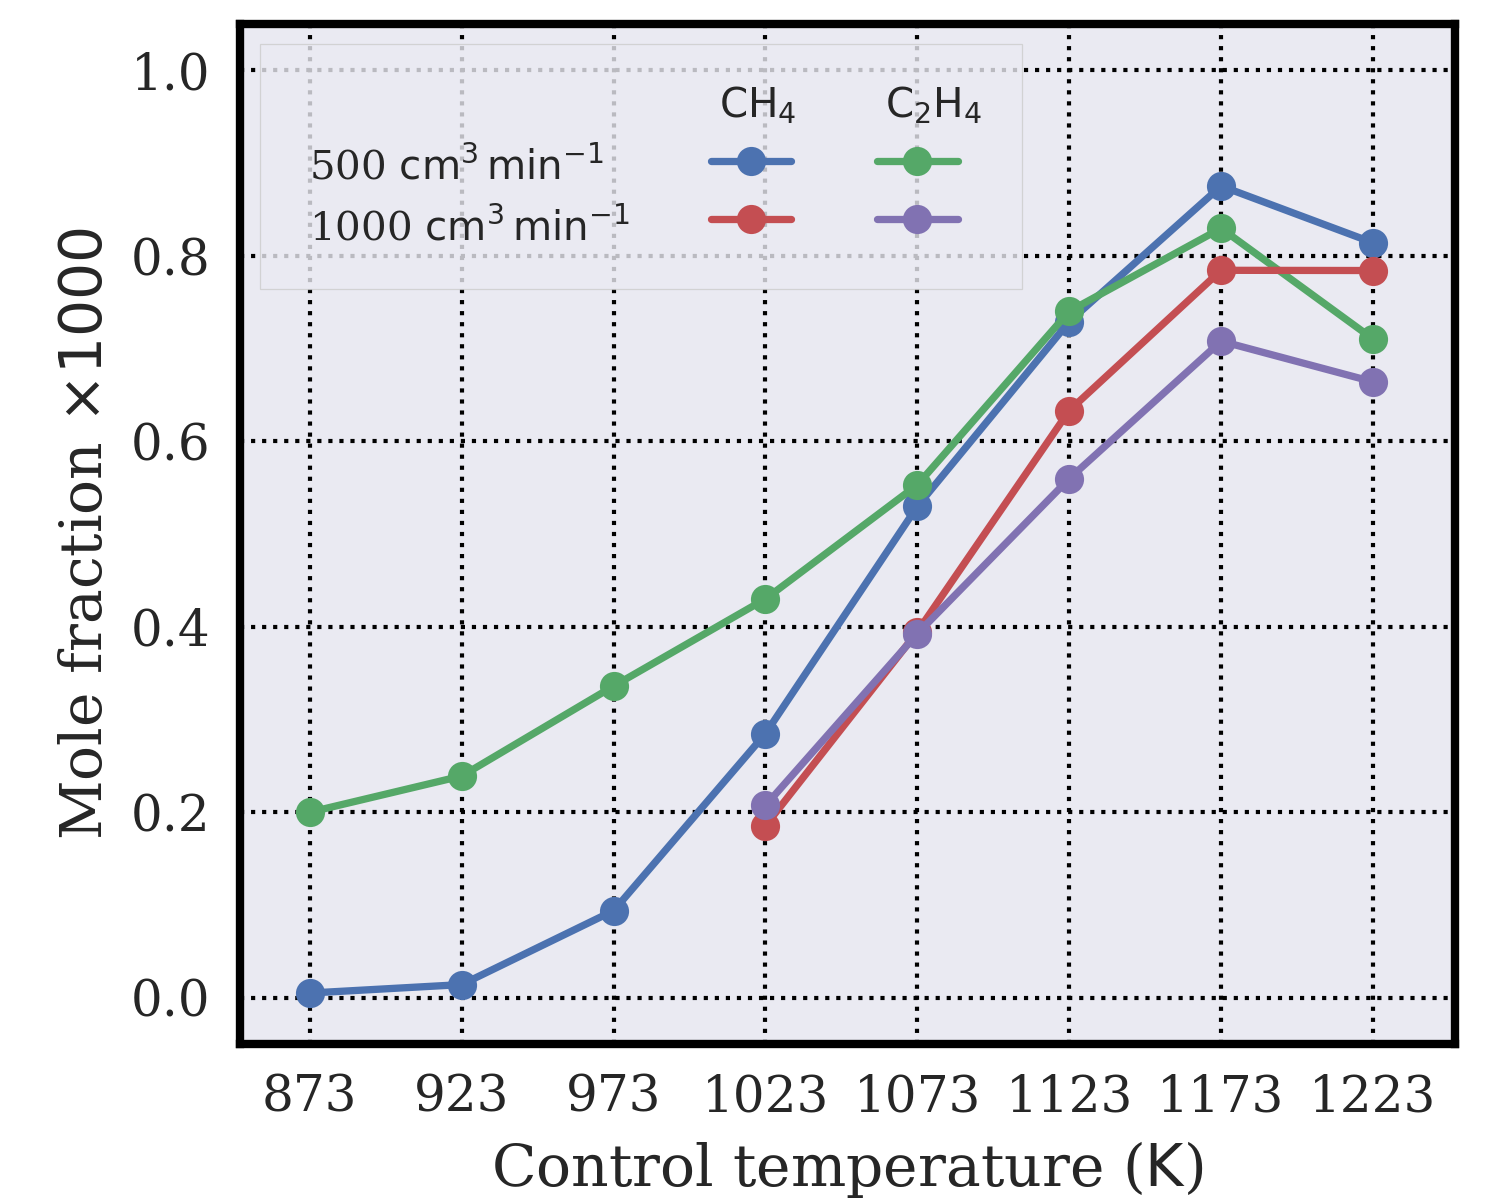
\includegraphics[width=\linewidth]
	{reworking/fractions_atmospheric_pressure_other}
	\caption{\label{fig:fractions-atmospheric-pressure-other}Measured mole fractions of \ch{CH4} and \ch{C2H4} at atmospheric pressure in terms of heated zone control temperature for different flow rates.}
\end{figure}

Above \SI{1023}{\kelvin}, Figure~\ref{fig:fractions-atmospheric-pressure-main}  provides measurements for both \SIlist{500;1000}{\sccm}. The main apparent effect of the increased flow rate is to \emph{delay} acetylene decomposition without any important change in reaction pathways since curves follow approximately parallel. This is due to the smaller residence time imposed by the higher flow rate, roughly half of the one at \SI{500}{\sccm}, as depicted in Figure~\ref{fig:residence-time-plot}. As expected, these curves show a laminar tubular flow reactor since globally Reynolds number $\mathrm{Re}<1$ with the given operating conditions.

%\begin{figure}[h]
%	\centering
%	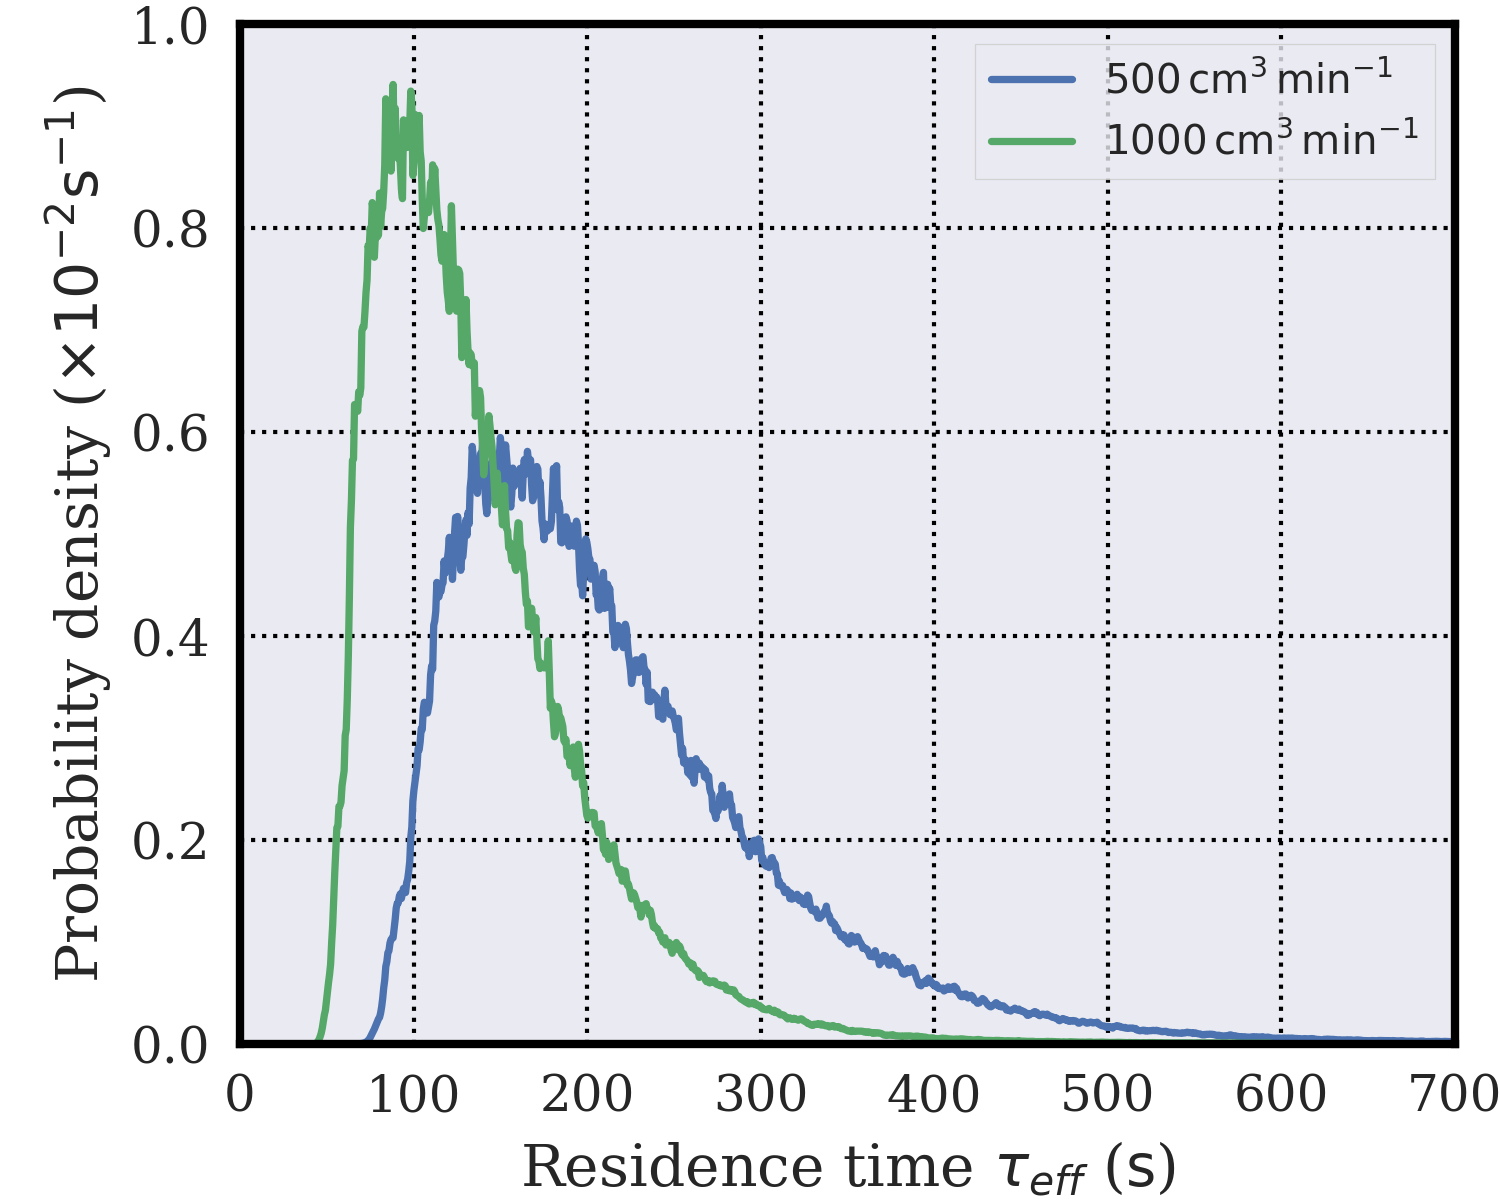
\includegraphics[width=\linewidth]{figures/residence_time_plot}
%	\caption{\label{fig:residence-time-plot}Atmospheric pressure residence time distributions for different total flow rates with control temperature set to \SI{1173}{\kelvin}.}
%\end{figure}

Mole balance analyses of the atoms composing the measured species are presented in Figure~\ref{fig:balance-atmospheric-pressure} and confirm ...

\begin{figure}[h]
	\centering
	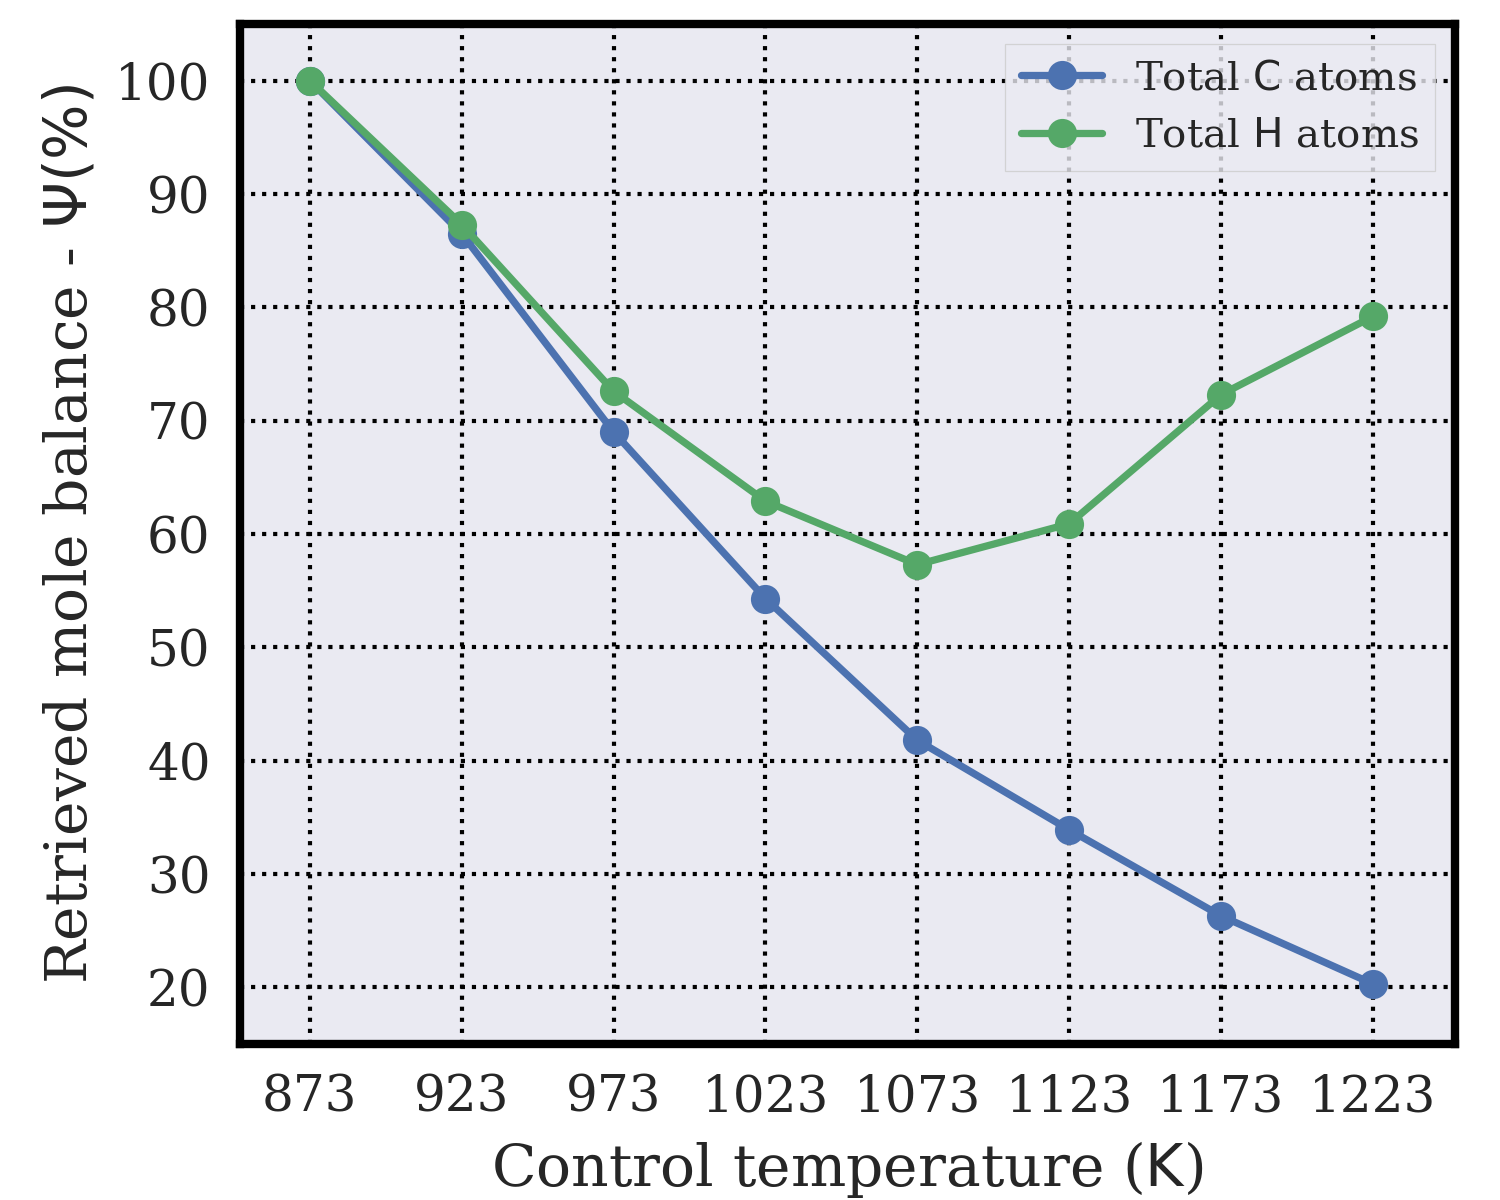
\includegraphics[width=\linewidth]
	{reworking/balance_atmospheric_pressure}
	\caption{\label{fig:balance-atmospheric-pressure}Retrieved percentage of carbon and hydrogen atoms at atmospheric pressure reactor outlet computed from species measurements presented in Figures~\ref{fig:fractions-atmospheric-pressure-main}~and~\ref{fig:fractions-atmospheric-pressure-other} (flow rate of \SI{500}{\cubic\centi\metre\per\minute}).}
\end{figure}

%TODO this should be here!
%\input{parts/table-results.tex}

\subsection{Low pressure decomposition}

\begin{figure}
	\centering
	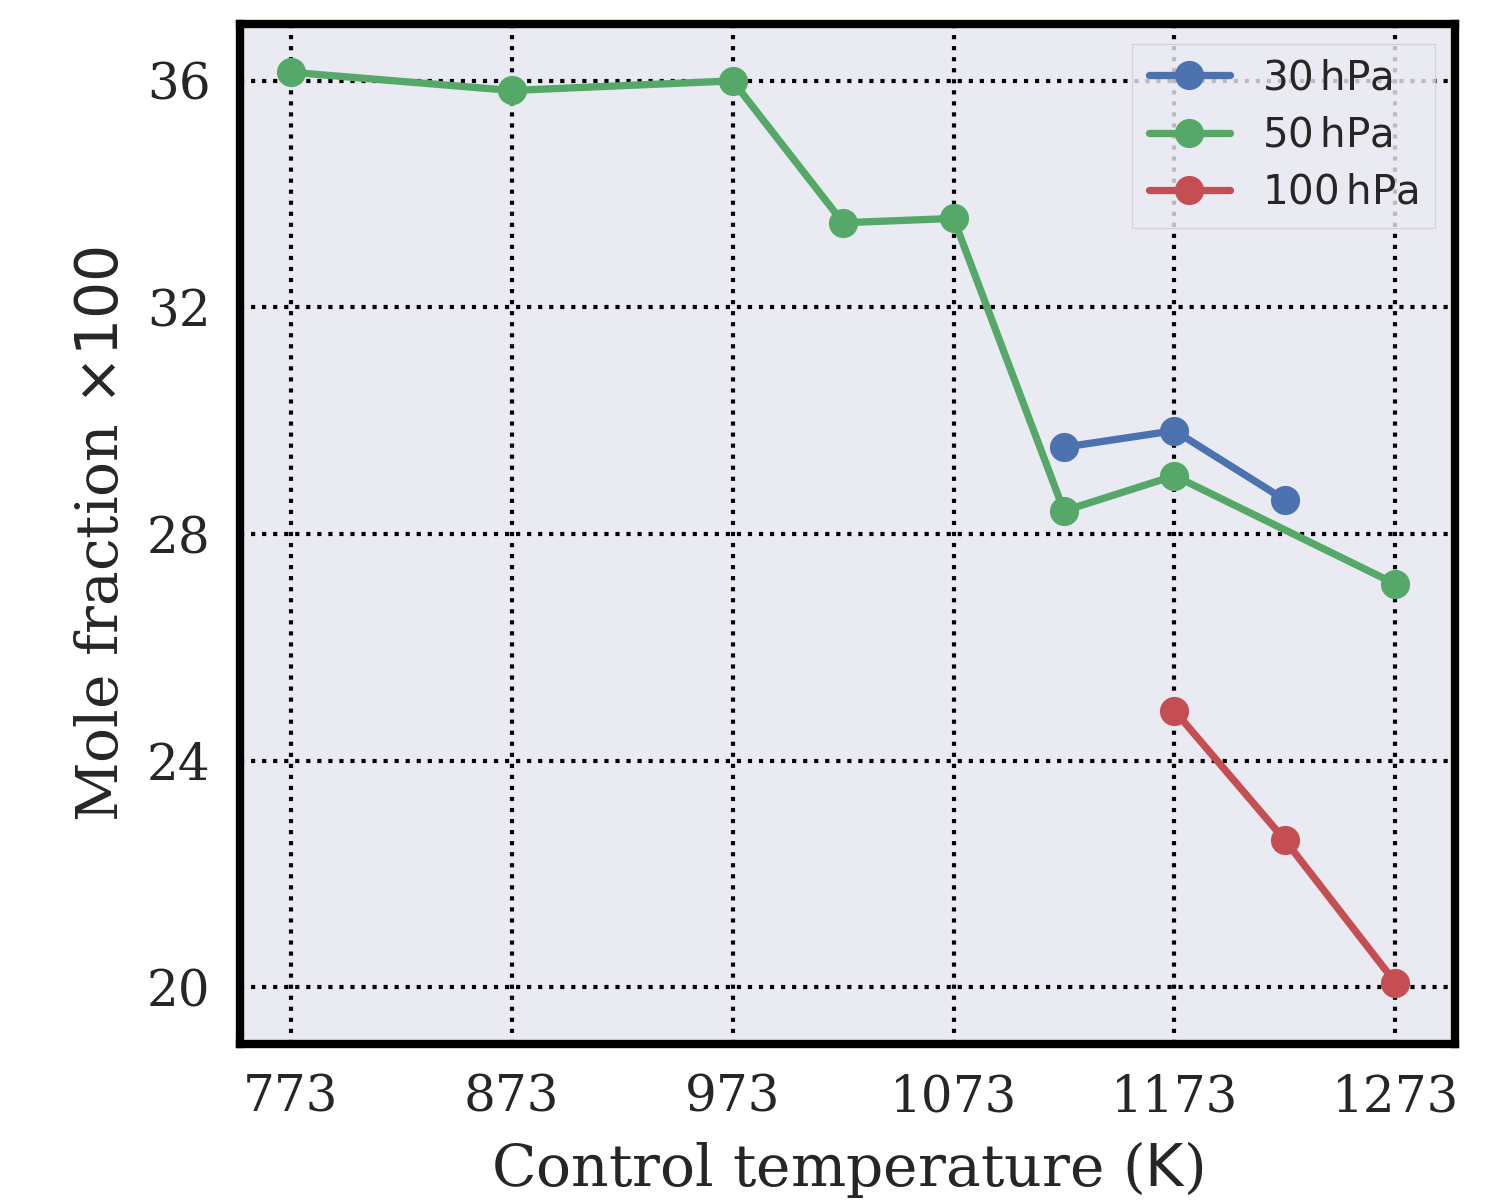
\includegraphics[width=\linewidth]
	{reworking/fractions_low_pressure}
	\caption{\label{fig:fractions-low-pressure}Measured mole fractions of \ch{C2H2} at different reduced pressures in terms of heated zone control temperature for a total inlet flow rate of \SI{222}{\cubic\centi\metre\per\minute} of \ch{N2 - 0.36 C2H2}.}
\end{figure}

\begin{table*}
	\caption{\label{tab-comparison-sim-exp}Comparison between experimental and simulated (PFR model) acetylene output fractions.}
\end{table*}

\subsection{Mechanism simplification}

\begin{figure}
	\caption{\label{fig:simplification-curves}Number of residual species against simplification threshold factor $\eta$.}
\end{figure}

\subsection{Numerical simulation}

\begin{figure}
	\caption{\label{fig:solution comparison}Comparison between full and simplified mechanisms of solution profiles along reactor axis for selected species.}
\end{figure}

\section{Conclusion}

\section*{Acknowledgments}

The authors are grateful to CNRS and IRT M2P for the financial support. We would also like to acknowledge the companies Safran, PSA Peugeot Citroën, Faurecia, ECM Technologies, Ascometal, Air Liquide, Airbus Helicopters, Arcelor Mittal, UTC Aerospace Systems and Poclain Hydraulics for the supply of raw materials and financial support through IRT M2P.

\begin{table*}
	\caption{\label{tab-sampling-conditions}Initial conditions for PSR solution sampling of solution space state for mechanism simplification.}
\end{table*}

\appendix
\section{Temperature profiles}
\begin{figure}
	\centering
	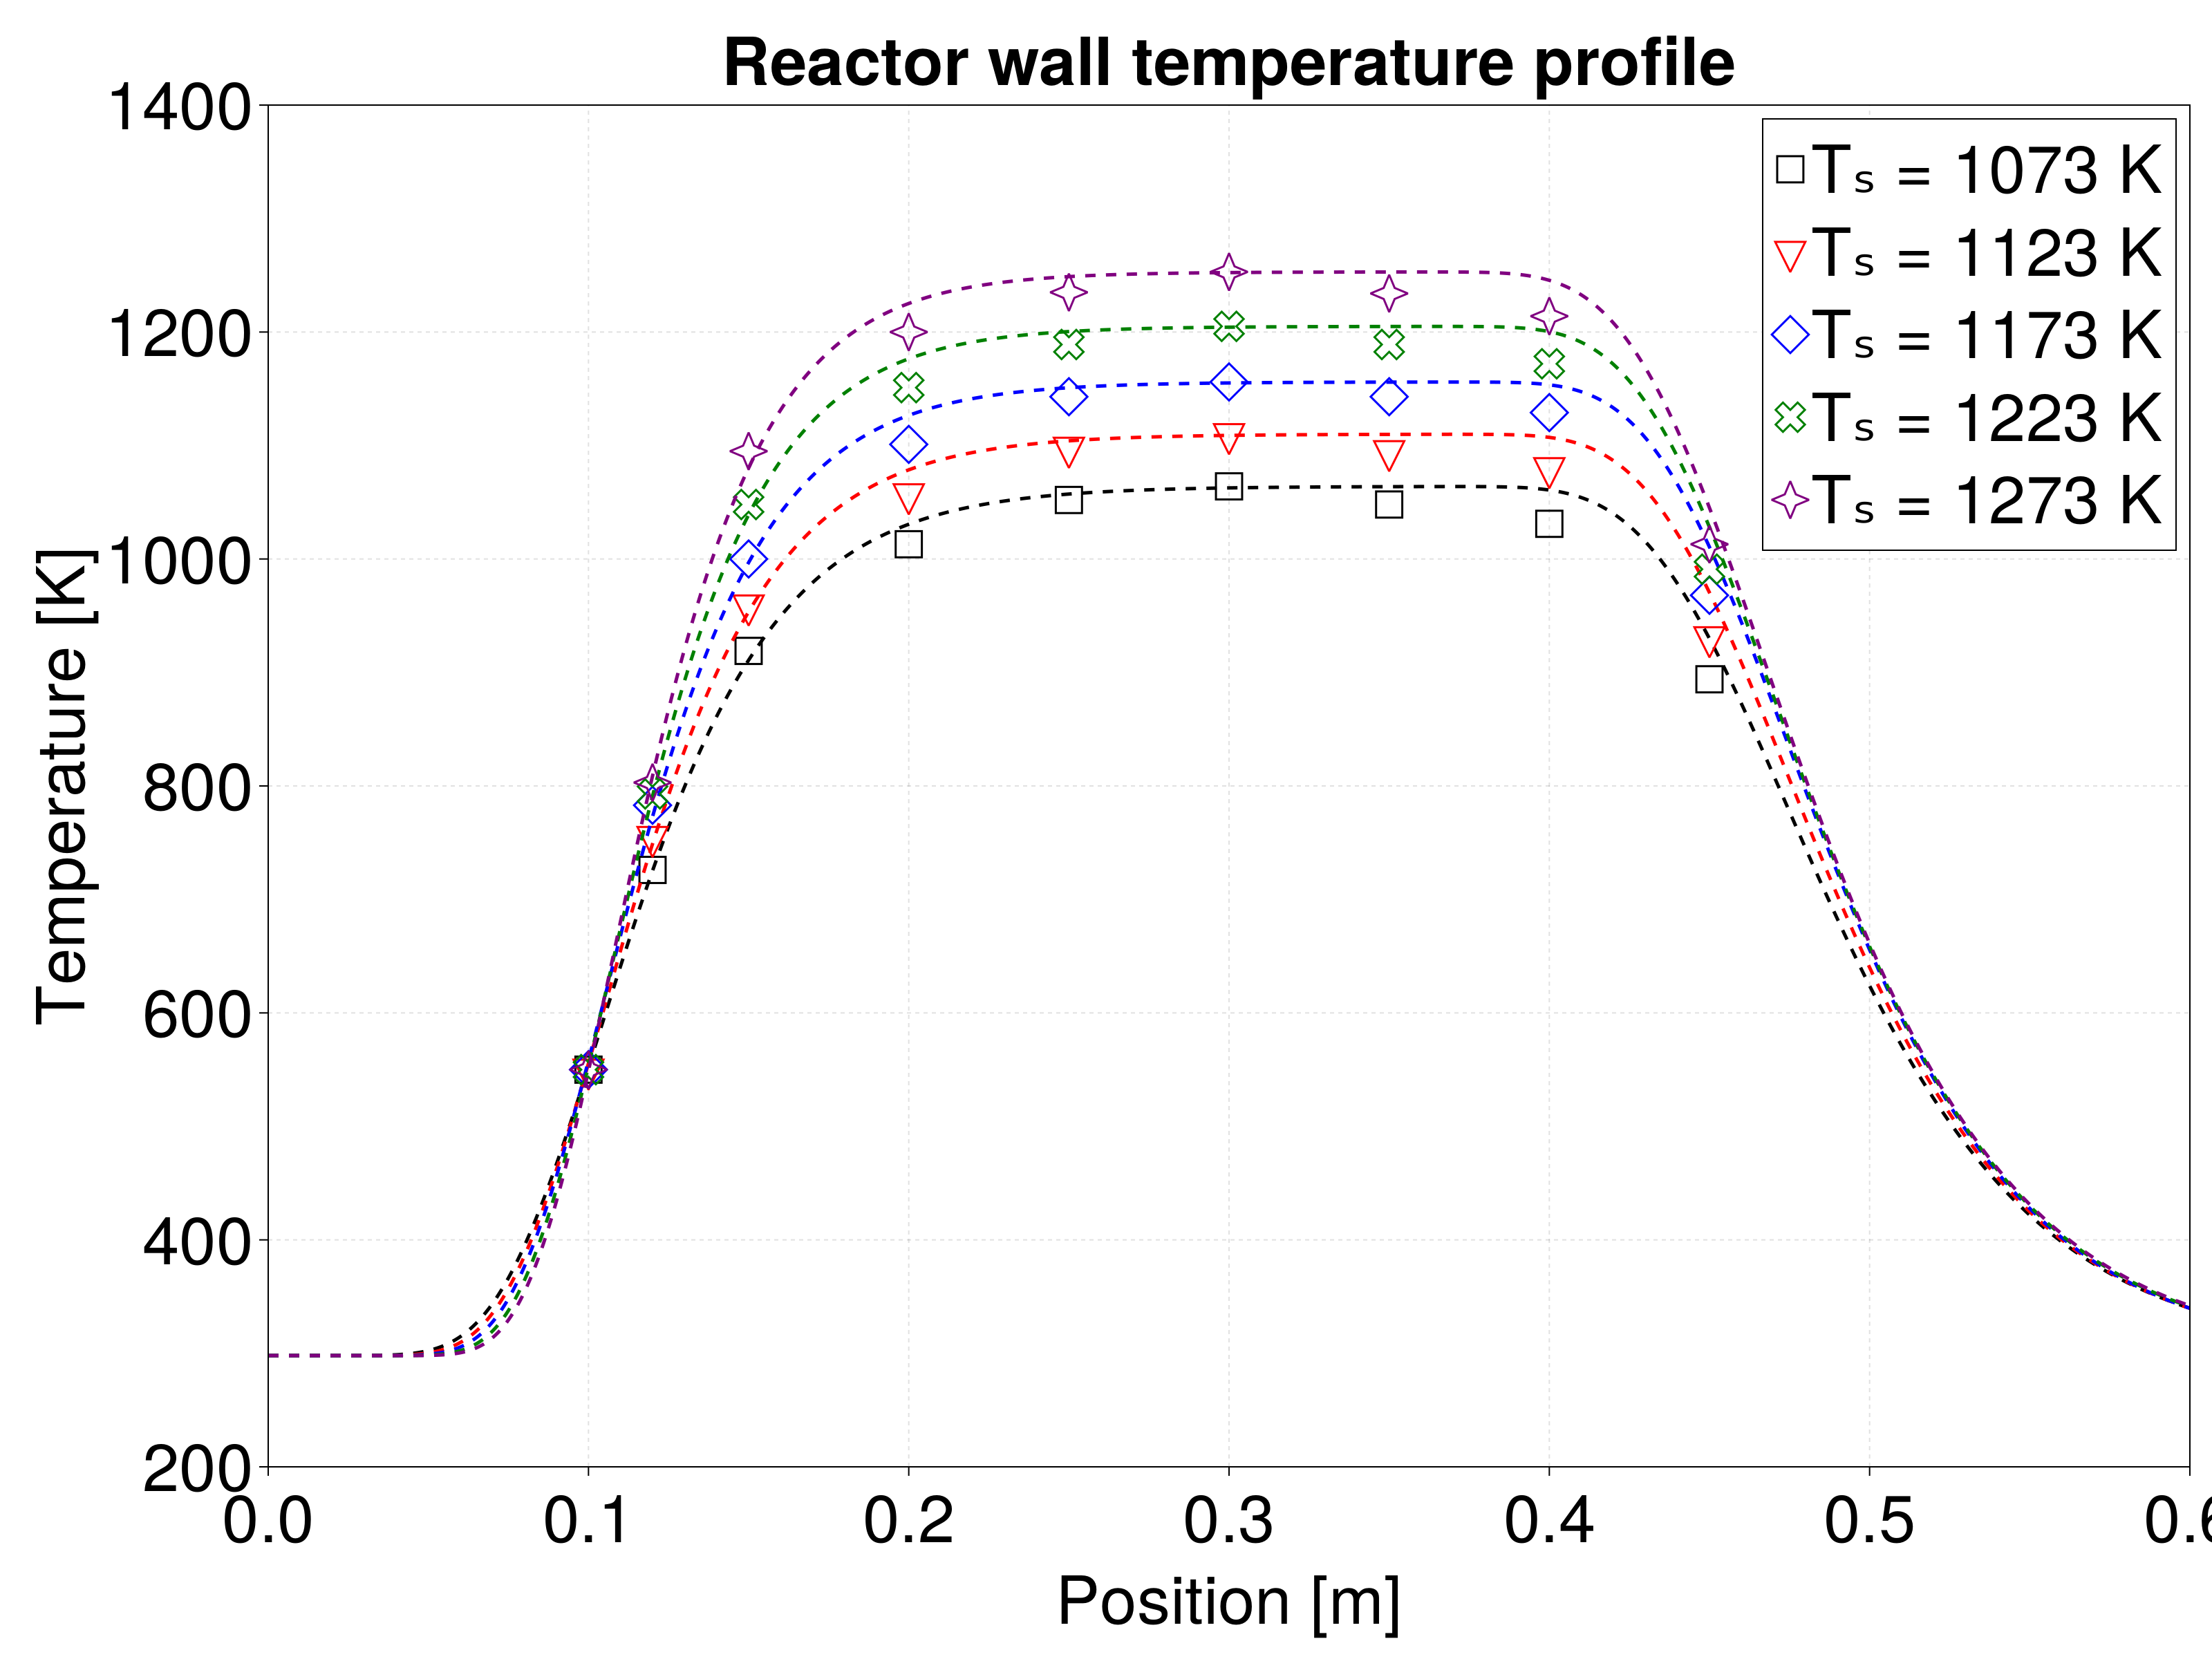
\includegraphics[width=\linewidth]{wall-temperature}
	\caption{\label{fig:temperature-profile}Measured wall temperature profiles along horizontal reactor axis for selected temperatures. Adjusted curves are provided as lines while actual measurements are depicted as dots.}
\end{figure}

\section{Simplified mechanism}

\begin{table*}
	\caption{\label{tab-species-to-kep}Species to keep for the skeletal mechanism obtained for acetylene pyrolysis from the mechanism by \citet{Norinaga2009}.}
\end{table*}


\section*{References}
\bibliography{article}

\end{document}